\documentclass{UoYCSproject}

\setlength{\marginparwidth}{2cm}
\usepackage{todonotes} % to be removed, used for adding markers for references needed
\usepackage{marginfix}

\usepackage[nohyperlinks]{acronym} % addition for acronyms page
\usepackage{amsmath} % for equation environments
\usepackage{algorithm} % for algorithm environments
\usepackage{algorithmic} % for algorithm content
\usepackage{listings} % for code listings
\usepackage{xcolor} % for colored text in listings
\usepackage{tikz} % for diagrams
\usetikzlibrary{positioning,shapes,arrows,fit,calc}
\usepackage{multirow} % for tables with merged rows
\usepackage{tabularx} % for tables with adjustable-width columns
\usepackage{hyperref}

% Configure listings
\lstset{
  basicstyle=\ttfamily\small,
  commentstyle=\color{gray},
  keywordstyle=\color{blue},
  stringstyle=\color{green!50!black},
  numbers=left,
  numberstyle=\tiny,
  numbersep=5pt,
  frame=single,
  breaklines=true,
  breakatwhitespace=false,
  showstringspaces=false
}

\addbibresource{bibliography.bib}
\author{Mischa}
\title{Identifying Images Generated by AI using Watermarks}
\date{Version 3.0, 2020-November}
\supervisor{Dimitar Kazakov}
\BSc

\dedication{
    To my parents, for their love and support.
}

\acknowledgements{
  I would like to thank my supervisors, Dimitar Kazakov and Dr. Kofi Appiah, for their guidance and support throughout this project.
}

% More definitions & declarations in example.ldf

\begin{document}
\pagenumbering{roman}
\maketitle
\listoffigures
\listoftables
% \renewcommand*{\lstlistlistingname}{List of Listings}
% \lstlistoflistings

% List of Acronyms used
\chapter*{List of Acronyms}
\addcontentsline{toc}{chapter}{List of Acronyms}
\begin{acronym}[XXXXX]  % Use longest acronym width to suppress error
  \acro{AI}{Artificial Intelligence}
  \acro{GAIM}{Generative AI Image Model}
  \acro{VAE}{Variational Autoencoder}
  \acro{GAN}{Generative Adversarial Network}
  \acro{DM}{Diffusion Model}
  \acro{LDM}{Latent Diffusion Model}
  \acro{RGB}{Red, Green, Blue}
  \acro{LSB}{Least Significant Bit}
  \acro{DCT}{Discrete Cosine Transform}
  \acro{DFT}{Discrete Fourier Transform}
  \acro{DWT}{Discrete Wavelet Transform}
  \acro{LPM}{Log-Polar Mapping}
  \acro{MSE}{Mean Squared Error}
  \acro{PSNR}{Peak Signal-to-Noise-Ratio}
  \acro{SSIM}{Structural Similarity Index Measure}
  \acro{NCC}{Normalised Cross-Correlation}
  \acro{BER}{Bit Error Rate}
  \acro{FID}{Fréchet Inception Distance}
  \acro{BCH}{Bose-Chaudhuri-Hocquenghem}
  \acro{CDF}{Cumulative Distribution Function}
  \acro{FPR}{False Positive Rate}
  \acro{TPR}{True Positive Rate}
  \acro{CLIP}{Contrastive Language-Image Pre-training}
  \acro{JPEG}{Joint Photographic Experts Group}
  \acro{CUDA}{Compute Unified Device Architecture}
  \acro{VRAM}{Video Random Access Memory}
  \acro{C2PA}{Coalition for Content Provenance and Authenticity}
  \acro{DDIM}{Denoising Diffusion Implicit Models}
\end{acronym}

\begin{summary}

\end{summary}


\begin{ethics}
This statement outlines the ethical considerations for this project, structured around the following principles: Avoidance of Harm, Informed Consent, and Data Protection.

\subsection*{Avoidance of Harm}
This project aims to explore technology that mitigates the potential harms of \ac{AI}-generated images. By enabling robust watermarking, this work helps combat misinformation (e.g., deepfakes), provides a mechanism for artists to receive attribution for their work, and aligns with regulatory demands for transparency in syntheticly generated media, such as the European Union \ac{AI} Act \cite{RegulationEU20242024}.

Potential risks have been considered and mitigated. The risk of malicious actors reverse engineering the watermark is addressed by focusing on robustness evaluation rather than vulnerability exploitation. The potential for misuse regarding privacy/surveilance is acknowledged; however, the project's scope is strictly limited to authenticity and attribution, not tracking individuals.

\subsection*{Informed Consent}
This project does not involve human participants. All experiments are conducted using publicly available datasets and open-source software, adhering to their respective licensing terms (e.g., Creative Commons for MS-COCO \cite{linMicrosoftCOCOCommon2015}, MIT License for Gaussian Shading source code \cite{__fubar__BsmhmmlfGaussianShading2025}). The research ensures transparency and reproducibility by documenting all methodologies and making evaluation scripts available.

\subsection*{Data Protection}
No personal or sensitive data was collected, processed, or stored. The datasets used (MS-COCO and Gustavosta prompts \cite{GustavostaStableDiffusionPromptsDatasets2023}) are publicly available for research and contain no personally identifiable information. All generated images and research data will only be retained as long as necessary to ensure reproducibility. The project adheres to responsible research practices, including minimising computational resources to reduce environmental impact.

Based on these considerations, formal ethical approval from the Physical Sciences Ethics Committee (PSEC) was not required. All ethical aspects have been discussed with the project supervisor, and the completed ethics checklist is available in Appendix \ref{app:EthicsChecklist}.
\end{ethics}


\chapter{Introduction}
\label{cha:Introduction}
\section{Motivation and Problem Statement}
The proliferation of powerful \acp{GAIM} such as Stable Diffusion \cite{rombachHighResolutionImageSynthesis2022}, DALL-E \cite{rameshZeroShotTexttoImageGeneration2021}, and Midjourney mark a significant technological leap, unlocking new possibilities in fields like content creation, design prototyping, and automation. However, the ease with which these models can generate highly realistic synthetic media introduces critical ethical and practical challenges, including the spread of misinformation \cite{ferraraGenAIHumanityNefarious2024}, copyright infringement, and a general erosion of trust in digital content. Furthermore, current rulings by the United States Copyright Office render purely \ac{AI}-generated images ineligible for copyright protection \cite{CopyrightRegistrationGuidance2023}.

In response, a clear consensus is forming around the need for establishing authenticity, attribution, and traceability mechanisms for synthetic media. Governmental bodies, including the White House through its 2023 Executive Order on \ac{AI} \cite{houseExecutiveOrderSafe2023} and the European Union via its 2024 AI Act \cite{RegulationEU20242024}, have mandated the use of techniques like invisible watermarking for synthetic content. Consequently, leading technology companies have begun integrating such solutions; notable examples include Google's SynthID \cite{IdentifyingAIgeneratedImages2024}, Microsoft's watermarking in Bing Image Creator \cite{BingPreviewRelease2023}, and Stability AI's watermarking methods for its models \cite{CompVisStablediffusion2024}.

The urgency for effective watermarking is further underscored by concerns surrounding the data used to train \acp{GAIM}. Artists have voiced concerns about the unauthorised use of their work \cite{ThousandsArtistsCondemn2024}, leading to \ac{AI}-generated images that mimic their unique styles without credit or compensation \cite{AndersenStabilityAI}. This has fueled the development of defensive techniques like Glaze \cite{shanGlazeProtectingArtists2023} and Nightshade \cite{shanNightshadePromptSpecificPoisoning2024}, which disrupt model training \cite{kurakinAdversarialExamplesPhysical2017}, highlighting the creative community's demand for control. While digital watermarking has a long history \cite{coxDigitalWatermarking2001}, its application to generative AI presents new challenges requires solutions that are integrated directly into the generation process. This project addresses the critical need for such a method, one that is imperceptible, robust against manipulation, capable of carrying attribution data without degrading image quality, and integrated within the generation process itself.

\section{Project Aims \& Scope}
The primary aim of this project is to investigate and evaluate the integration of digital watermarking within \ac{AI} image generation models to address the critical issues of \textbf{authenticity, attribution, traceability, and copyright protection}. To this end, the project will conduct a thorough evaluation of the Gaussian Shading watermarking algorithm, a state-of-the-art, training-free technique designed for \acp{LDM}.

To achieve this, the following objectives have been set:
\begin{enumerate}
    \item To conduct a focused review of modern watermarking techniques to identify the current state-of-the-art, justify the selection of Gaussian Shading, and position it within the field.
    \item To implement the Gaussian Shading algorithm within a standard \ac{GAIM} framework, specifically Stable Diffusion v2.1.
    \item To design and execute a comprehensive evaluation framework to test the watermark's imperceptibility and its robustness against a suite of common digital attacks.
    \item To analyse the results, assessing the crucial trade-offs between robustness, imperceptibility, and data capacity, and compare against published benchmarks to critically assess the performance and viability of Gaussian Shading as a practical watermarking solution.
\end{enumerate}

This project seeks to answer the following research questions:
\begin{itemize}
    \item To what extent can the Gaussian Shading method provide robust watermarking against a standard set of digital attacks, including compression, noise, and geometric transformations?
    \item What is the trade-off between watermark robustness and image quality? Can the method's "performance-lossless" claim be substantiated using distribution based metrics like \ac{FID} and \ac{CLIP} score?
    \item How does the performance of Gaussian Shading compare to other leading in-generation watermarking techniques.
\end{itemize}

The key contribution of this project is a rigorous and independent empirical evaluation of the Gaussian Shading watermarking method. By providing detailed performance data and a direct comparison to established benchmarks, this work offers valuable insights for the development of responsible and traceable \ac{AI} generated image generation systems.

\section{Dissertation Structure}
The remainder of this dissertation is organised as follows: Chapter 2 reviews the literature on generative models and watermarking, focusing on the state-of-the-art techniques that lead to the selection of Gaussian Shading. Chapter 3 details the methodology, system architecture, and the specific framework used for implementation and evaluation. Chapter 4 presents the results of the empirical evaluation, analysing the imperceptibility and robustness of the implemented solution. Finally, Chapter 5 concludes the dissertation, summarising the findings in relation to the research questions, discussing the study's limitations, and potential directions for future work.


\chapter{Literature Review}
\label{cha:Literature Review}
\section{Background}

\subsection{Generative Models in AI Image Generation}
Generative images have revolutionised the \ac{AI} field by enabling the creation of new data that closely resembles the training data. The three primary generative models used in \ac{AI} image generation being: \acp{GAN}, \acp{VAE}, and \acp{DM}.

\subsubsection{Variational Autoencoders (\acp{VAE})}
\acp{VAE} were first defined in 2013 by Kingma et al. \cite{kingmaAutoEncodingVariationalBayes2022} and Rezende et al. \cite{rezendeStochasticBackpropagationApproximate2014}. \acp{VAE} are probabilistic generative models that learn a latent space representation of input data. They consist of an encoder and a decoder, which work together to reconstruct input data from a compressed latent space. Watermarking in \acp{VAE} could involve perturbing latent space to insert information \cite{guoFreqMarkInvisibleImage2024}.

\subsubsection{Generative Adversarial Networks}
\acp{GAN}, proposed by Goodfellow et al. \cite{goodfellowGenerativeAdversarialNetworks2014} in 2014. \acp{GAN} consist of two neural networks: A generator, and a discriminator. The generator takes an input of random noise and generates an image by reassembling the real data distribution; The discriminator seeks to differentiate between real and generated images. The competing nature of the model helps in improving the quality of images generated over time. However, images generated are sensitive to perturbations \cite{alfarraRobustnessQualityMeasures2022}. Therefore, adding a watermark could degrade the quality of the image.

\subsubsection{Diffusion Models}
\acp{DM} were first introduced in 2015 by Sohl-Dickstein et al. \cite{sohl-dicksteinDeepUnsupervisedLearning2015} and popularised in 2020 by Ho et al. \cite{hoDenoisingDiffusionProbabilistic2020}. Unlike \acp{GAN} and \acp{VAE}, \acp{DM} generate images by iteratively denoising a random noise pattern, producing high quality images with fine details. The challenge in watermarking \acp{DM} lies in ensuring the watermark does not interfere with the denoising process in order to preserve image quality. \acp{LDM} such as Stable Diffusion, extend the concept of diffusion by performing the denoising process in a latent space rather than directly in pixel space, allowing for more efficient training and inference, as well as improved image quality \cite{rombachHighResolutionImageSynthesis2022}. In \acp{LDM}, a \ac{VAE} is used to compress the image to into a lower-dimensional latent space, which is then denoised iteratively to generate the final image.

\subsection{Applications and Motivations for Watermarking in the AI Era}
The rise of \acp{GAIM} has created an urgent need for robust watermarking solutions to address several key challenges.

\subsubsection{Preventing Training Data Contamination and Model Collapse}
Many \acp{GAIM} are trained on large datasets scraped from the internet. A significant risk in this process is "model collapse", where models are inadvertently trained on their own synthetic outputs or those from other models. This can lead to a feedback loop that degrades the quality and diversity of generated content over time \cite{bohacekNepotisticallyTrainedGenerativeAI2023}. Watermarking \ac{AI} generated images can mitigate this by marking these synthetic outputs, allowing them to be filtered out of future training datasets, thereby preserving the integrity of the training data.

\subsubsection{Attribution, Traceability, and Content Authenticity}
Watermarks can act as digital fingerprints for \ac{AI} generated images, enabling robust attribution and traceability. Depending on the implementation, a watermark could encode information about the originating model, the user, or the time of generation. This is vital for accountability, particularly when addressing the use of copyrighted material in training data or the distribution of malicious content. Initiatives like the \ac{C2PA}, backed by major technology firms, aim to standardise how this provenance information is embedded and read, creating a framework for digital content certification \cite{ContentCredentialsC2PA}. An effective watermarking scheme is therefore essential for copyright protection, verifying ownership, and ensuring the authenticity of digital media in an age of prolific \ac{AI} generation \cite{jiangWatermarkbasedDetectionAttribution2024}.

\section{Digital Watermarking Techniques}
\subsection{Traditional Spatial Domain Watermarking}
Spatial domain watermarking involves embedding watermarks directly into the pixel values. These methods are straightforward, easy to implement, and computationally efficient. However, are typically less resistant to attacks such as compression and transformations.

\subsubsection{Least Significant Bit (\ac{LSB}) Modification}
A common technique to embed a watermark information into randomly chosen pixels' \ac{LSB}. The \ac{LSB} is changed as to not affect the image quality as it contains less important information. However, it is trivial for an attacker to change all \ac{LSB} bits to 1 to modify the watermark. To address the problems with \ac{LSB} watermarking, improvements have been made. One such improvement embeds data not only to the \ac{LSB} but also higher planes. Moreover, a 2-3-3 embedding technique \cite{manjulaNovelHashBased2015} distributes the watermark across the \ac{RGB} channels of a pixel. This approach results in minimal perceptual distortion while achieving better embedding capacity and robustness.

\subsubsection{Patch-based or Block-Based techniques}
Proposed by Bender et al. \cite{benderTechniquesDataHiding1996} This method involves randomly picking $n$ pairs of image points $A,B$ where the image data in $A$ is darkened, while is brightened in $B$. This method offers decent robustness in exchange for capacity. \cite{saqibSpatialFrequencyDomain2017}

\subsection{Traditional Frequency (Transform) Domain Watermarking}
These techniques embed watermark information within the frequency domain of an image after a transformation. This approach spreads the watermark information throughout the image in ways that are less perceptible to the human eye and more resilient to common attacks compared to spatial methods.

\subsubsection{Discrete Cosine Transform}
\ac{DCT} watermarking embeds watermark information into an images frequency coefficients after transforming it from the spatial to the frequency domain. This leverages energy compaction, where the majority of an image's visual information is represented by lower-frequency coefficients, while higher-frequency coefficients capture finer image details. A common approach is block-based \ac{DCT}, where the image is divided into smaller non-overlapping blocks, \ac{DCT} is then applied to each block. Mid-frequency coefficients are typically chosen, balancing imperceptibility and robustness. Modifying low-frequency coefficients can lead to more noticeable distortions, while high-frequency coefficients are more susceptible to compression and noise attacks. Block-based \ac{DCT} is particularly suitable for \ac{JPEG} compression, a prevalent image compression technique which is also block-based \cite{wallaceJPEGStillPicture1991}. By embedding watermarks in \ac{DCT} coefficients compatible with \ac{JPEG}'s compression algorithm, the watermark can survive compression without significant degradation \cite{borsImageWatermarkingUsing1996}. Alternatively, global \ac{DCT} applies the transformation to the entire image rather than individual blocks. This offers greater robustness against attacks, but is more computationally intensive and less compatible with block-based compression techniques such as \ac{JPEG}.

The robustness of \ac{DCT}-based watermarking comes from the ability to embed data in perceptually significant regions of an image, therefore being less likely to be removed by common image processing operations. However, \ac{DCT} based watermarking methods struggle with maintaining robustness against geometric attacks such as scaling and rotation due to inherently not accounting for spatial transformations \cite{fazliRobustImageWatermarking2016}. From this hybrid techniques combining \ac{DCT} with other transformations have arisen \cite{abdulrahmanNovelHybridDCT2019}.

\subsubsection{Discrete Fourier Transform}
Similar to \ac{DCT} watermarking, \ac{DFT} embeds watermark information into an images frequency domain by transforming it from the spatial domain to the frequency domain, but using the \ac{DFT} which decomposes an image into sinusoidal components of varying frequencies, represented as complex-valued coefficients corresponding to magnitude and phase. These coefficients describe the global frequency characteristics of the image, making \ac{DFT}-based watermarking inherently robust against various image processing operations and certain geometric transformations.

\ac{LPM} transforms the image into log-polar coordinates before applying \ac{DFT}. This mapping converts scaling and rotation into linear translations in the frequency domain, enabling efficient watermark extraction after significant geometric transformations \cite{zhengRSTinvariantDigitalImage2003}.

\subsubsection{Discrete Wavelet Transform}
A \ac{DWT} is any wavelet transform that decomposes a signal into wavelets, offering local analysis in both the time and frequency domains. Unlike \ac{DFT}, which analyses global frequency count, and \ac{DCT} which can operate globally or block-based, \ac{DWT} inherently supports multi-resolution analysis by examining signals at different scales. This dual localisation makes \ac{DWT} particularly effective for image watermarking, as it can capture coarse and fine image details simultaneously.

\subsubsection{Applications to AI-Generated Images}
Traditional frequency domain methods (DCT, DWT) represent conventional image watermarking approaches that operate in the frequency domain. While well-established and widely used for natural images, these techniques are generic post-processing methods that don't specifically leverage the properties of the AI generation processes. Their application remains relatively unexplored in recent LDM-specific literature compared to direct latent modification approaches that are purposefully designed for AI-generated content.

\subsection{Post-Generation Methods}
Methods like HiDDeN \cite{zhuHiDDeNHidingData2018} and FreqMark \cite{guoFreqMarkInvisibleImage2024} demonstrate impressive results, they are designed as post-generation solutions that can be applied to any image, regardless of its source. This makes them less specifically tailored to the unique characteristics and requirements of AI-generated content.
\subsubsection{HiDDeN}
One promising advancement in watermarking is the HiDDeN framework \cite{zhuHiDDeNHidingData2018}. HiDDeN leverages the sensitivity of deep neural networks to small perturbations in input images to encode information, making it a robust solution for watermarking.

The HiDDeN framework comprises three main components: an encoder, a decoder, and an adversary network. The encoder receives an image and a message string, outputting an encoded image that incorporates the watermark. The decoder attempts to reconstruct the original message from the encoded image, while the adversary network predicts whether a given image contains an encoded watermark, providing adversarial loss to enhance the quality of the encoded images.

The adversarial training enhances the watermark's resilience against numerous attacks. The deep leaning approach allows for a more flexible watermark embedding,

\subsection{Modern Watermarking for AI-Generated Images}
Recent advancements have focused on integrating watermarks directly into the generative process of \acp{DM} and \acp{LDM}, offering greater robustness and imperceptibility compared to traditional post-processing methods.

\subsubsection{Tree-Ring}
Tree-Ring \cite{wenTreeRingsWatermarksInvisible2023} is a notable in-generation technique for \acp{DM}. It operates by embedding a watermark signal into the initial noise vector ($z_{T}$) before the diffusion process begins. The core idea is that the deterministic nature of \ac{DDIM} inversion allows for the retrieval of the initial noise vector from the final generated image. By comparing the recovered noise with the known watermark signal, the presence of the watermark can be detected. While effective for detection, its original design is primarily for a 1-bit watermark, which limits its viability for use other than binary watermark detection.

\subsubsection{Stable Signature}
Stable Signature \cite{fernandezStableSignatureRooting2023b} is a watermarking approach designed specifically for \acp{LDM}. Instead of modifying the initial noise, this method fine-tunes the model's autoencoder (\ac{VAE}). The \ac{VAE}'s decoder is trained to embed a specific watermark pattern into the generated image's pixel space while the encoder is trained to be robust to its presence. By embedding the watermark directly into the model's architecture, Stable Signature aims to create a watermark that is deeply integrated with the image's content and thus more resilient to post-processing attacks.

\subsubsection{Gaussian Shading}
Gaussian Shading \cite{yangGaussianShadingProvable2024} is a training-free, performance-lossless watermarking technique for \acp{LDM}. Unlike methods that require model fine-tuning, Gaussian Shading is a plug-and-play solution that modifies the initial latent sampling step. The watermark is mapped to a latent representation that follows a standard Gaussian distribution, making it statistically indistinguishable from a non-watermarked latent vector. This ensures that the watermarking process does not degrade the performance of the generative model. The watermark is embedded by diffusing the bits across the latent dimensions and then using a distribution-preserving sampling method. Extraction is achieved through \ac{DDIM} inversion to retrieve an estimate of the initial latent, from which the watermark can be recovered. The authors provide theoretical proof of its performance-lossless nature and demonstrate high robustness against common attacks, outperforming many existing methods.

\subsubsection{Comparative Analysis}
To provide a clear overview, Table \ref{tab:watermarking_comparison} compares the different watermarking techniques discussed.

\begin{table}[htb]
\caption{Comparison of Digital Watermarking Techniques.}
\label{tab:watermarking_comparison}
\begin{center}
\resizebox{\textwidth}{!}{%
\begin{tabular}{|l|l|l|l|l|l|}
\hline
\textbf{Technique} & \textbf{Domain} & \textbf{Robustness} & \textbf{Imperceptibility} & \textbf{Capacity} & \textbf{Training-Free} \\ \hline
\ac{LSB} & Spatial & Low & High & High & Yes \\ \hline
\ac{DCT} & Frequency & Medium & Medium & Medium & Yes \\ \hline
\ac{DWT} & Frequency & High & High & Medium & Yes \\ \hline
Tree-Ring & Latent (\ac{DM}) & High & High & Low (1-bit) & Yes \\ \hline
Stable Signature & Latent (\ac{LDM}) & High & High & High & No \\ \hline
Gaussian Shading & Latent (\ac{LDM}) & High & High (Provably Lossless) & High & Yes \\ \hline
\end{tabular}%
}
\end{center}
\end{table}

\section{Watermarking Optimisations and Enhancements}
\subsection{Perceptual Masking}
Perceptual masking exploits the characteristics of human vision by embedding watermarks into regions of an image where the changes will be less noticeable. For example, areas with high texture or edges rather than flat or uniform areas.

\section{Watermarking Challenges and Evaluation}
A successful watermarking scheme must be robust against a variety of attacks designed to remove or degrade the embedded information. Furthermore, its performance must be quantifiable using standard evaluation metrics.

\subsection{Attacks on Watermarks}
Watermarks are susceptible to a wide range of attacks, which can be broadly categorised as follows:
\textbf{Removal Attacks:} These are designed to completely eliminate the watermark signal from the image. This can include denoising filters or adversarial attacks specifically trained to target and erase the watermark.
\textbf{Geometric Attacks:} These attacks alter the geometry of the image, which can desynchronise the detector. Common examples include rotation, scaling, cropping, and translation.
\textbf{Signal Processing Attacks:} These are common image manipulations that can unintentionally degrade or destroy the watermark. This category includes lossy compression (e.g., \ac{JPEG}), noise addition (e.g., Gaussian noise), and filtering (e.g., blurring).

A robust watermarking system must be able to withstand a combination of these attacks to be considered effective in real-world scenarios.

\subsection{Metrics for Evaluation}
To objectively assess the performance of a watermarking technique, a set of standard metrics is used to measure three key properties:
\begin{itemize}
    \item \textbf{Imperceptibility:} This measures the visual distortion introduced by the watermark. For traditional watermarking methods, commonly quantified using pixel level metrics like \ac{PSNR} and \ac{SSIM}. However, for latent space watermarking methods like Gaussian Shading, distribution-based metrics such as \ac{FID} and \ac{CLIP} Score are more appropriate. Lower \ac{FID} values mean the distribution of watermarked images is closer to that of the original images, while similar \ac{CLIP} scores indicate that the semantic content of the images remain consistent with the original prompts.
    \item \textbf{Robustness:} This is a measure of the watermark's ability to survive attacks. Typically evaluated by calculating the \ac{BER} between the original and extracted watermark message after an attack has been applied. A lower \ac{BER} indicates better robustness.
    \item \textbf{Capacity:} This refers to the amount of information (in bits) that can be embedded within the watermark. There is often a trade-off between capacity, robustness, and imperceptibility.
\end{itemize}
These metrics provide the foundation for the experimental evaluation framework described in the next chapter.

\chapter{Methodology}
\label{cha:Methodology}

This chapter details the approach taken to investigate, implement, and evaluate the Gaussian Shading watermarking technique for \ac{AI} generated images. It covers the research strategy, the selection of the specific watermarking technique from available literature, a detailed experimental design, and the comprehensive framework for evaluation. The methodology will provide a rigorous assessment that enables direct comparison with state-of-the-art techniques while operating within the feasibility constraints of an undergraduate project.

\section{Research Approach}
\label{sec:ResearchApproach}

This study employs a \textbf{quantitative empirical evaluation} methodology to assess the performance of Gaussian Shading watermarking. The approach is aligned with established benchmarks in the watermarking literature, specifically following the evaluation protocols used by Tree-Ring \cite{wenTreeRingsWatermarksInvisible2023} and Stable Signature \cite{fernandezStableSignatureRooting2023b}, enabling direct comparison without requiring re-implementation of competing methods.

The selection of \acp{LDM} as the primary architecture is justified by their current dominance in high quality image generation and the availability of open source implementations \cite{dhariwalDiffusionModelsBeat2021}. Specifically, Stable Diffusion \cite{rombachHighResolutionImageSynthesis2022} is chosen due to its open source nature \cite{CompVisStablediffusion2024}, widespread adoption in research, and existing watermarking literature within its framework \cite{fernandezStableSignatureRooting2023b, zhaoRecipeWatermarkingDiffusion2023a, zhangAttackResilientImageWatermarking2024}.

\section{Watermarking Technique Selection}
\label{sec:WatermarkingTechniqueSelection}

The primary goal is to embed imperceptible watermarks that facilitate traceability and attribution. Based on the literature review, several approaches are viable, particularly those designed for or adaptable to \acp{LDM}. Latent space modification techniques like Stable Signature \cite{fernandezStableSignatureRooting2023b}, Tree-Ring \cite{wenTreeRingsWatermarksInvisible2023}, LaWa \cite{rezaeiLaWaUsingLatent2024}, ZoDiac \cite{zhangAttackResilientImageWatermarking2024}, and WMAdapter \cite{ciWMAdapterAddingWaterMark2024} propose embedding the watermark within the latent space during the image generation process. This approach is specifically designed for AI image generation, as it integrates directly with the generative model's architecture and workflow.

The final selection of the watermarking technique is based on the following criteria:
\begin{enumerate}
    \item \textbf{Suitability for LDM Integration:} How readily the technique can be integrated into the Stable Diffusion architecture.
    \item \textbf{Robustness Potential:} Theoretical and empirical evidence from literature regarding resistance to common image manipulations.
    \item \textbf{Capacity for Attribution Data:} Ability to embed a sufficient payload for traceability purposes \cite{jiangWatermarkbasedDetectionAttribution2024}.
    \item \textbf{Imperceptibility:} Maintaining high visual quality of the generated images.
    \item \textbf{Implementation Feasibility:} Availability of reference implementations or clarity of the proposed algorithm within the project timeframe.
\end{enumerate}

Based on these criteria, Gaussian Shading \cite{yangGaussianShadingProvable2024} was selected. Its approach modifies the initial latent sampling process, offering direct integration (Criterion 1). A key advantage is its provably performance-lossless nature, meaning it does not require model fine-tuning and aims to preserve the original model's output quality (Criteria 1, 4, 5). The original paper reports high robustness and good capacity (Criteria 2 \& 3), making it a strong candidate. While other latent space methods like Stable Signature \cite{fernandezStableSignatureRooting2023b} or Tree-Ring \cite{wenTreeRingsWatermarksInvisible2023} (originally designed primarily for 1-bit capacity, limiting its suitability for detailed attribution data under Criterion 3) also offer strong integration, Gaussian Shading's advantage for this project lies with it being performance-lossless without needing model fine-tuning or architectural changes (Criterion 5). This simplifies implementation and ensures the watermark minimally impacts the generative capabilities of the base Stable Diffusion model (Criterion 4), compared to approaches that might require adjustments to the \ac{VAE} or U-Net.


\section{Experimental Design}
\label{sec:ExperimentalDesign}

\subsection{Standard Evaluation Protocol}
\label{subsec:StandardEvaluationProtocol}

To ensure reproducible and comparable results, the evaluation follows a standardised protocol:

\begin{itemize}
    \item \textbf{Generative Model:} Stable Diffusion v2.1-base
    \item \textbf{Image Resolution:} 512$\times$512 pixels (standard for SD v2.1)
    \item \textbf{Guidance Scale:} 7.5 (classifier-free guidance strength)
    \item \textbf{Inference Steps:} 50 (using DPMSolver++ scheduler)
    \item \textbf{Precision:} Float16 for memory efficiency
    \item \textbf{Batch Size:} 1 (for reproducibility and memory constraints)
\end{itemize}

These parameters align with established benchmarks and ensure compatibility with the RTX 2070 Super GPU constraints (8GB \ac{VRAM}) while maintaining generation quality.

\subsection{Dataset Selection and Justification}
\label{subsec:DatasetSelection}

The evaluation employs a two-tier dataset strategy to balance comprehensive assessment with computational feasibility. The primary dataset for imperceptibility and baseline quality analysis is derived from the MS-COCO \cite{linMicrosoftCOCOCommon2015} 2017 validation set captions. From this, a subset of 1000 diverse prompts was curated to ensure a representative sample for calculating the \ac{FID} score, aligning with standard evaluation practices in the literature.

For the robustness evaluation, a different prompt set was created from the \texttt{Gustavosta/Stable-Diffusion-Prompts} \cite{GustavostaStableDiffusionPromptsDatasets2023} collection. This dataset is known for its diverse and challenging prompts. A subset of 200 prompts was selected to cover a wide range of categories, including portraits, landscapes, objects, and abstract concepts. This reduction to 200 prompts was a made to ensure the feasibility of executing the suite of 12 attack configurations on each generated image within the time and hardware constraints of the project, while still providing sufficient data for analysis.

\subsection{Watermark Configuration}
\label{subsec:WatermarkConfiguration}

The watermark implementation follows the Gaussian Shading specification with a 256-bit capacity. For empirical testing, the payload consists of random binary strings per generation to facilitate robust \ac{BER} analysis; in practice, this would contain attribution data (generation ID, model identifier, timestamp). The payload is then encrypted using a ChaCha20 stream cipher with random key/nonce per image before embedding. Standard diffusion parameters (\texttt{channel\_copy = 1}, \texttt{hw\_copy = 8}) are used as specified in \cite{yangGaussianShadingProvable2024}. The detection threshold targets an \ac{FPR} of $10^{-6}$ for statistical significance. Practically, deployment would also incorporate error correction codes (e.g., \ac{BCH} codes) before embedding to enhance robustness against channel noise and attacks.

\section{System Architecture}
\label{sec:SystemArchitecture}

The Gaussian Shading watermarking system operates through two primary pipelines: embedding and extraction. Figure \ref{fig:system_architecture} illustrates the complete architecture of the system, highlighting the key components and data flow.

\subsection{Embedding Pipeline}
The \textbf{embedding pipeline} integrates watermarking directly into the image generation process:

\begin{enumerate}
    \item \textbf{Text Encoding:} The process begins with a text prompt that is encoded using the \ac{CLIP} text encoder to produce conditioning vectors.
    
    \item \textbf{Watermark Preparation:} The watermark message $s$ (a binary string) is diffused across latent dimensions to obtain $s_{d}$, creating redundant copies for robustness. The diffused watermark $s_{d}$ is then encrypted with a ChaCha20 stream cipher using a secret key $K$ to produce $m$.
    
    \item \textbf{Distribution-Preserving Sampling:} The core innovation occurs during initial latent sampling. Instead of standard sampling $z_{T} \sim \mathcal{N}(0, I)$, the method uses distribution-preserving sampling based on $m$ using a Gaussian quantile function and uniform random sampling. This ensures the watermarked latent maintains the same statistical properties as a non-watermarked latent.
    
    \item \textbf{Denoising Process:} The watermarked latent $z_{T}$ undergoes standard 50-step diffusion denoising guided by the conditioning vectors.
    
    \item \textbf{Image Decoding:} Finally, the \ac{VAE} decoder transforms the denoised latent representation into the final watermarked image in pixel space.
\end{enumerate}

\subsection{Extraction Pipeline}
The \textbf{extraction pipeline} reverses the embedding process to recover the watermark:

\begin{enumerate}
    \item \textbf{Latent Encoding:} The watermarked image is encoded using the \ac{VAE} encoder to produce a latent representation $z_{0}'$.
    
    \item \textbf{\ac{DDIM} Inversion:} A deterministic \ac{DDIM} inversion process with 50 steps is applied to estimate the initial noise $z_{T}'$ that would have generated the image.
    
    \item \textbf{Watermark Recovery:} Inverse sampling logic (Gaussian \ac{CDF}) extracts a randomized watermark estimate $m'$ from $z_{T}'$, which is decrypted with key $K$ to recover the diffused watermark estimate $s_{d}'$.
    
    \item \textbf{Bit Reconstruction:} A reduction/voting mechanism across the diffused copies recovers the final watermark estimate $s'$, enabling binary classification between watermarked and non-watermarked images based on the recovered bits.
\end{enumerate}

The architecture is designed to be modular, allowing for adjustments to parameters such as the number of diffusion steps, watermark length, and diffusion redundancy factors without requiring structural changes.

\begin{figure}[htb]
    \centering
    \resizebox{\textwidth}{!}{%
\begin{tikzpicture}[
    node distance=0.8cm,
    % Compact styles to fit within page margins
    embedding/.style={rectangle, draw, rounded corners, minimum width=1.8cm, minimum height=0.5cm, align=center, fill=blue!15, font=\scriptsize},
    extraction/.style={rectangle, draw, rounded corners, minimum width=1.8cm, minimum height=0.5cm, align=center, fill=green!15, font=\scriptsize},
    algorithm/.style={rectangle, draw, rounded corners, minimum width=2.2cm, minimum height=0.6cm, align=center, fill=yellow!20, font=\scriptsize},
    data/.style={rectangle, draw, rounded corners, minimum width=1.5cm, minimum height=0.5cm, align=center, fill=gray!10, font=\scriptsize},
    arrow/.style={->,>=stealth},
    section/.style={draw, rounded corners, fill=gray!5, inner sep=4pt}
]

% EMBEDDING PIPELINE (Top Section)
\node[section, label={[anchor=north west, font=\scriptsize]north west:\textbf{Embedding Pipeline}}] (embedding_section) at (0,0) {
    \begin{tikzpicture}[node distance=0.6cm]
        % Row 1
        \node[data] (prompt) {Text Prompt};
        \node[embedding, right=of prompt] (clip_encoder) {CLIP\\Encoder};
        \node[data, right=of clip_encoder] (text_emb) {Text Emb.};
        
        % Row 2
        \node[data, below=of prompt] (watermark_bits) {256-bit WM};
        \node[algorithm, right=of watermark_bits] (diffusion) {WM Diffusion\\$ch=1, hw=8$};
        \node[algorithm, right=of diffusion] (encryption) {ChaCha20};
        
        % Row 3
        \node[algorithm, below=0.8cm of diffusion] (gaussian_shading) {Gaussian Shading\\$z_T^{(w)} = \Phi^{-1}(...)$};
        
        % Row 4
        \node[data, below=of gaussian_shading] (watermarked_latent) {WM Latent};
        \node[embedding, right=of watermarked_latent] (unet) {U-Net\\50 steps};
        \node[embedding, right=of unet] (vae_dec) {VAE Dec.};
        
        % Final output
        \node[data, below=of unet] (wm_image) {WM Image};
        
        % Simple direct connections to avoid overlaps
        \draw[arrow] (prompt) -- (clip_encoder);
        \draw[arrow] (clip_encoder) -- (text_emb);
        \draw[arrow] (watermark_bits) -- (diffusion);
        \draw[arrow] (diffusion) -- (encryption);
        \draw[arrow] (encryption) |- (gaussian_shading);
        \draw[arrow] (text_emb) |- (gaussian_shading);
        \draw[arrow] (gaussian_shading) -- (watermarked_latent);
        \draw[arrow] (watermarked_latent) -- (unet);
        \draw[arrow] (unet) -- (vae_dec);
        \draw[arrow] (vae_dec) |- (wm_image);
    \end{tikzpicture}
};

% EXTRACTION PIPELINE (Bottom Section)
\node[section, below=1cm of embedding_section, label={[anchor=north west, font=\scriptsize]north west:\textbf{Extraction Pipeline}}] (extraction_section) {
    \begin{tikzpicture}[node distance=0.6cm]
        % Row 1
        \node[data] (attacked_input) {Test Image};
        \node[extraction, right=of attacked_input] (vae_encoder) {VAE Enc.};
        \node[data, right=of vae_encoder] (latent_repr) {Latent $z_0'$};
        
        % Row 2
        \node[algorithm, below=of vae_encoder] (ddim_inversion) {DDIM Inversion\\50 steps};
        \node[data, right=of ddim_inversion] (estimated_latent) {Est. $z_T'$};
        
        % Row 3
        \node[algorithm, below=of ddim_inversion] (inverse_sampling) {Inverse\\Sampling};
        \node[extraction, right=of inverse_sampling] (decryption) {ChaCha20\\Dec.};
        
        % Row 4
        \node[extraction, below=of inverse_sampling] (majority_voting) {Majority\\Vote};
        \node[data, right=of majority_voting] (extracted_watermark) {Extract. $s'$};
        
        % Row 5
        \node[algorithm, below=of majority_voting] (ber_calculation) {BER Calc.};
        \node[data, right=of ber_calculation] (detection_result) {Pass/Fail};
        
        % Simple connections
        \draw[arrow] (attacked_input) -- (vae_encoder);
        \draw[arrow] (vae_encoder) -- (latent_repr);
        \draw[arrow] (latent_repr) |- (ddim_inversion);
        \draw[arrow] (ddim_inversion) -- (estimated_latent);
        \draw[arrow] (estimated_latent) |- (inverse_sampling);
        \draw[arrow] (inverse_sampling) -- (decryption);
        \draw[arrow] (decryption) |- (majority_voting);
        \draw[arrow] (majority_voting) -- (extracted_watermark);
        \draw[arrow] (extracted_watermark) |- (ber_calculation);
        \draw[arrow] (ber_calculation) -- (detection_result);
    \end{tikzpicture}
};

% Connect sections
\draw[arrow, thick] (embedding_section.south) -- (extraction_section.north);

\end{tikzpicture}
}
    \caption{Complete system architecture diagram showing the embedding pipeline (top) and extraction pipeline (bottom). The embedding pipeline integrates watermarking into the generation process by modifying the initial latent sampling, while the extraction pipeline uses DDIM inversion to recover the watermark.}
    \label{fig:system_architecture}
\end{figure}

\section{Implementation Details}
\label{sec:ImplementationDetails}

\subsection{Technical Environment}
\label{subsec:TechnicalEnvironment}

The implementation utilises an NVIDIA RTX 2070 Super (8GB \ac{VRAM}) with \ac{CUDA} 11.7, running Python 3.8 with PyTorch 1.13+ and Diffusers 0.11.1. Key dependencies include transformers (4.21.0) for \ac{CLIP} text encoding, accelerate for memory optimisation, scipy for statistical functions, and pycryptodome for ChaCha20 cryptographic operations. The 8GB \ac{VRAM} constraint necessitates memory efficiency strategies: float16 precision reduces memory footprint by 50\%, sequential processing prevents out-of-memory errors, and gradient checkpointing enables processing of 512×512 images. Memory allocation is optimised through PyTorch's attention implementation and careful tensor lifecycle management during \ac{DDIM} inversion.

\subsection{Gaussian Shading Implementation}
\label{subsec:GaussianShadingImplementation}

The implementation follows the algorithm specification from \cite{yangGaussianShadingProvable2024}, The method consists of three key components: watermark diffusion, distribution preserving sampling, and DDIM inversion for extraction.

\subsubsection{Watermark Diffusion}
The watermark message $s \in \{0,1\}^m$ undergoes an initial diffusion process across its latent dimensions to enhance robustness. This process generates multiple copies of each bit across different dimensions, defined as $s_{d} = \text{Diffuse}(s, \text{channel\_copy}, \text{hw\_copy})$. Where $\text{channel\_copy}$ determines how many copies are made across channel dimensions, and $\text{hw\_copy}$ controls copies across spatial dimensions. This redundancy is important for robustness, as it allows for majority voting during extraction even if some dimensions are corrupted by attacks. The diffused watermark $s_d$ is then encrypted using ChaCha20 stream cipher with a secret key $K$ to produce the encrypted watermark $m$: $m = \text{Encrypt}(s_d, K)$

\subsubsection{Distribution Preserving Sampling}
A key part of Gaussian Shading is the distribution preserving sampling technique. In standard diffusion models, the initial latent is sampled from a standard normal distribution:

\begin{equation}
z_{T} \sim \mathcal{N}(0, I) \text{ (standard)}
\end{equation}

For watermarking, this sampling is modified to embed the encrypted watermark while maintaining the same statistical distribution:

\begin{equation}
z_{T}^{(w)} = \Phi^{-1}(U \cdot \Phi(z_{T}) + (1-U) \cdot \Phi(z_{T}^{(ref)})) \text{ (watermarked)}
\end{equation}

where:
\begin{itemize}
    \item $\Phi$ is the standard normal \ac{CDF}
    \item $\Phi^{-1}$ is the inverse \ac{CDF} (quantile function)
    \item $U$ is a uniform random variable in $[0,1]$
    \item $z_{T}^{(ref)}$ is a reference latent that encodes the encrypted watermark bits
\end{itemize}

This approach ensures that $z_{T}^{(w)}$ follows the same distribution as $z_{T}$, making the watermark statistically undetectable and preserving the generative model's performance. The implementation uses the error function (erf) and its inverse for efficient computation of the normal \ac{CDF} and quantile functions.

\subsubsection{\ac{DDIM} Inversion for Extraction}
The extraction process uses deterministic \ac{DDIM} inversion with 50 steps to estimate the initial latent. The algorithm is:

\begin{algorithm}
\caption{\ac{DDIM} Inversion for Watermark Extraction}
\begin{algorithmic}[1]
\REQUIRE Watermarked image $x$, number of steps $T$
\ENSURE Estimated initial latent $\hat{z}_T$
\STATE $z_0 \gets \text{VAE\_Encoder}(x)$ \COMMENT{Encode image to latent space}
\FOR{$t = 1$ to $T$}
    \STATE $\epsilon_\theta \gets \text{U-Net}(z_{t-1}, t-1)$ \COMMENT{Predict noise}
    \STATE $z_t \gets \text{DDIM\_Step}(z_{t-1}, \epsilon_\theta, t-1, t)$ \COMMENT{Reverse diffusion step}
\ENDFOR
\RETURN $z_T$
\end{algorithmic}
\end{algorithm}

Where $\text{DDIM\_Step}$ implements the deterministic reverse diffusion process according to the \ac{DDIM} formulation. Once the initial latent $\hat{z}_{T}$ is recovered, the watermark is extracted by applying the inverse of the distribution preserving sampling process: $\hat{m} = \text{Extract}(\hat{z}_{T}, K)$

The extracted watermark $\hat{m}$ is then decrypted and the diffused bits are combined through majority voting to recover the original message $\hat{s}$.

\subsubsection{Memory Optimization Techniques}
The implementation incorporates several memory optimization strategies to operate within the 8GB VRAM constraint:

\begin{itemize}
    \item \textbf{Half-precision arithmetic:} All tensors use float16 precision, reducing memory footprint by half compared to float32.
    \item \textbf{Sequential processing:} Images are processed one at a time rather than in batches to avoid memory spikes.
    \item \textbf{Efficient tensor management:} Careful attention to tensor lifecycle, explicitly freeing unused tensors and using in-place operations where possible.
    \item \textbf{Optimised attention implementation:} Using PyTorch's attention implementation to reduce memory footprint of transformer blocks in the U-Net.
\end{itemize}

These optimisations enable processing of $512\times512$ images on the specified hardware without compromising the quality of the watermarking process.

\section{Evaluation Framework}
\label{sec:EvaluationFramework}

\subsection{Attack Suite Configuration}
\label{subsec:AttackSuiteConfiguration}

The robustness evaluation employs a comprehensive attack suite designed to test common image processing operations:

\begin{table}[htb]
\caption{Attack Configuration Parameters}
\label{tab:attack_parameters}
\begin{center}
\begin{tabular}{|l|l|l|}
\hline
\textbf{Attack Type} & \textbf{Parameters} & \textbf{Configurations} \\
\hline
\ac{JPEG} Compression & Quality Factor & 90, 75, 50, 25 \\
\hline
Gaussian Noise & Standard Deviation & 0.01, 0.03, 0.05 \\
\hline
Gaussian Blur & Kernel Radius & 2, 4 \\
\hline
Brightness Adjustment & Multiplication Factor & 0.5, 2.0 \\
\hline
Random Crop & Retention Ratio & 0.8 \\
\hline
\end{tabular}
\end{center}
\end{table}

This configuration yields 12 attack scenarios, each evaluated on 200 images, totaling 2400 robustness experiments. The parameter ranges are selected to align with previous watermarking studies while covering mild to severe attack intensities.

\subsection{Evaluation Metrics}
\label{subsec:EvaluationMetrics}

The evaluation framework employs three metric categories.

While traditional metrics like \ac{PSNR} and \ac{SSIM} are common for assessing imperceptibility, they are not the primary metrics for this evaluation. The Gaussian Shading technique operates by altering the initial latent sample ($z_T$). As such, even when using an the same seed, the watermarked and non-watermarked images are inherently distinct at the pixel level, as they are slightly modified versions of one another. Applying pixel level metrics in this context is not appropriate, as they would report significant differences that do not reflect perceptual similarity.

Therefore, distribution based metrics are more appropriate. The \ac{FID} score is used to compare the statistical distributions of the entire set of 1000 watermarked images against the 1000 non-watermarked images, providing a more meaningful measure of the watermark's overall impact on the model's output distribution. Additionally, the \ac{CLIP} score is used to ensure that the semantic content of the generated images remains consistent with the original prompt, further validating the watermark's imperceptibility.

\textbf{Imperceptibility metrics} \ac{FID} for distribution preservation, and \ac{CLIP} Score for semantic similarity between prompts and generated images. \textbf{Robustness metrics} comprise \ac{BER} as the primary robustness measure, \ac{TPR} for detection accuracy at fixed \ac{FPR}, and overall detection accuracy for binary classification performance.

\subsection{Comparative Analysis Strategy}
\label{subsec:ComparativeAnalysisStrategy}

Rather than implementing competing methods, the evaluation strategy employs \textbf{benchmark extraction} from published literature:

\begin{enumerate}
    \item \textbf{Literature Analysis:} Extract performance metrics from Tree-Ring \cite{wenTreeRingsWatermarksInvisible2023} and Stable Signature \cite{fernandezStableSignatureRooting2023b} papers.
    \item \textbf{Standardised Comparison:} Align evaluation datasets and attack parameters with published benchmarks.
    \item \textbf{Statistical Analysis:} Report confidence intervals and significance tests where applicable.
    \item \textbf{Performance Tables:} Create comparative tables showing relative performance across methods.
\end{enumerate}

This approach enables rigorous comparison while remaining feasible within project constraints.

\subsection{Statistical Rigor and Reproducibility}
\label{subsec:StatisticalRigor}

Scientific validity is ensured through deterministic random number generation with fixed seeds for reproducibility, statistically sufficient sample sizes (n=200 per attack, n=1000 for \ac{FID}), 95\% confidence intervals for key metrics, and comprehensive documentation of all code and hyperparameters under version control.

\subsection{Success Criteria and Thresholds}
\label{subsec:SuccessCriteria}

The evaluation sets a clear success criteria to assess Gaussian Shading's viability. \textbf{Imperceptibility thresholds} require \ac{FID} $<$ 5.0 (indicating minimal distribution shift between watermarked and non-watermarked images) and \ac{CLIP} Score difference $<$ 0.05 (indicating preservation of semantic content). \textbf{Robustness thresholds} require \ac{BER} $<$ 0.1 for mild attacks (\ac{JPEG} QF $\geq$ 75), \ac{BER} $<$ 0.25 for moderate attacks (\ac{JPEG} QF $\geq$ 50), and \ac{TPR} $>$ 0.9 at \ac{FPR} = $10^{-6}$. These derived thresholds from the literature provide objective criteria for evaluating the performance lossless claims of Gaussian Shading.

The methodology balances comprehensive evaluation with practical constraints, ensuring that results are both scientifically valid and directly comparable to existing literature while remaining achievable within undergraduate project scope and hardware limitations.


\chapter{Results}
\label{cha:Results}

This chapter presents the empirical results of the evaluation, focusing on the two key performance areas for a watermarking system: imperceptibility and robustness. The findings are analysed to address the research questions concerning the viability of Gaussian Shading as a practical solution for \ac{AI}-generated media.

\section{Baseline Performance and Imperceptibility}
The first phase of the evaluation assessed the impact of the watermark on the output quality of the Stable Diffusion model. The goal was to empirically test the "performance-lossless" claim of the Gaussian Shading method using both semantic and distributional metrics.

Visually, as shown in Figure \ref{fig:visual_comparison}, the watermarked images are indistinguishable from their non-watermarked counterparts. This qualitative assessment is the first indication of the watermark's high imperceptibility. To quantify this, the \ac{CLIP} score, which measures the semantic similarity between the text prompt and the generated image, shows a negligible difference of 0.0008 between the watermarked (0.3091) and non-watermarked (0.3099) image sets. This is well within the success threshold of 0.05, confirming that the watermark does not degrade the semantic content of the generated images.

However, the \ac{FID} score presents a different story. The calculated score of 47.83, shown in Table \ref{tab:imperceptibility_metrics}, is nearly an order of magnitude higher than the success threshold of 5.0. The \ac{FID} score measures the difference in the statistical distributions of the two image sets. This high value indicates that while the images look the same and represent the same content, the underlying distribution of pixel values has been significantly altered by the watermarking process. This result presents a critical challenge to the "performance-lossless" claim, suggesting that while visually and semantically lossless, the method is not statistically lossless. It is important to note that this evaluation was conducted on 1,000 images, whereas the original paper used 5,000; \ac{FID} is known to be sensitive to sample size, which may contribute to the discrepancy.

\begin{table}[htb]
    \caption{Imperceptibility and Distributional Metrics.}
    \label{tab:imperceptibility_metrics}
    \begin{center}
    \begin{tabular}{|l|c|c|c|c|}
    \hline
    \textbf{Metric} & \textbf{Ground Truth} & \textbf{Watermarked} & \textbf{Success Threshold} & \textbf{Verdict} \\ \hline
    \ac{CLIP} Score & 0.3099 & 0.3091 & \textless 0.05 difference & \textbf{Pass} \\ \hline
    \ac{FID} Score & - & 47.83 & \textless 5.0 & \textbf{Fail} \\ \hline
    \end{tabular}
    \end{center}
\end{table}

\begin{figure}[htb]
    \centering
    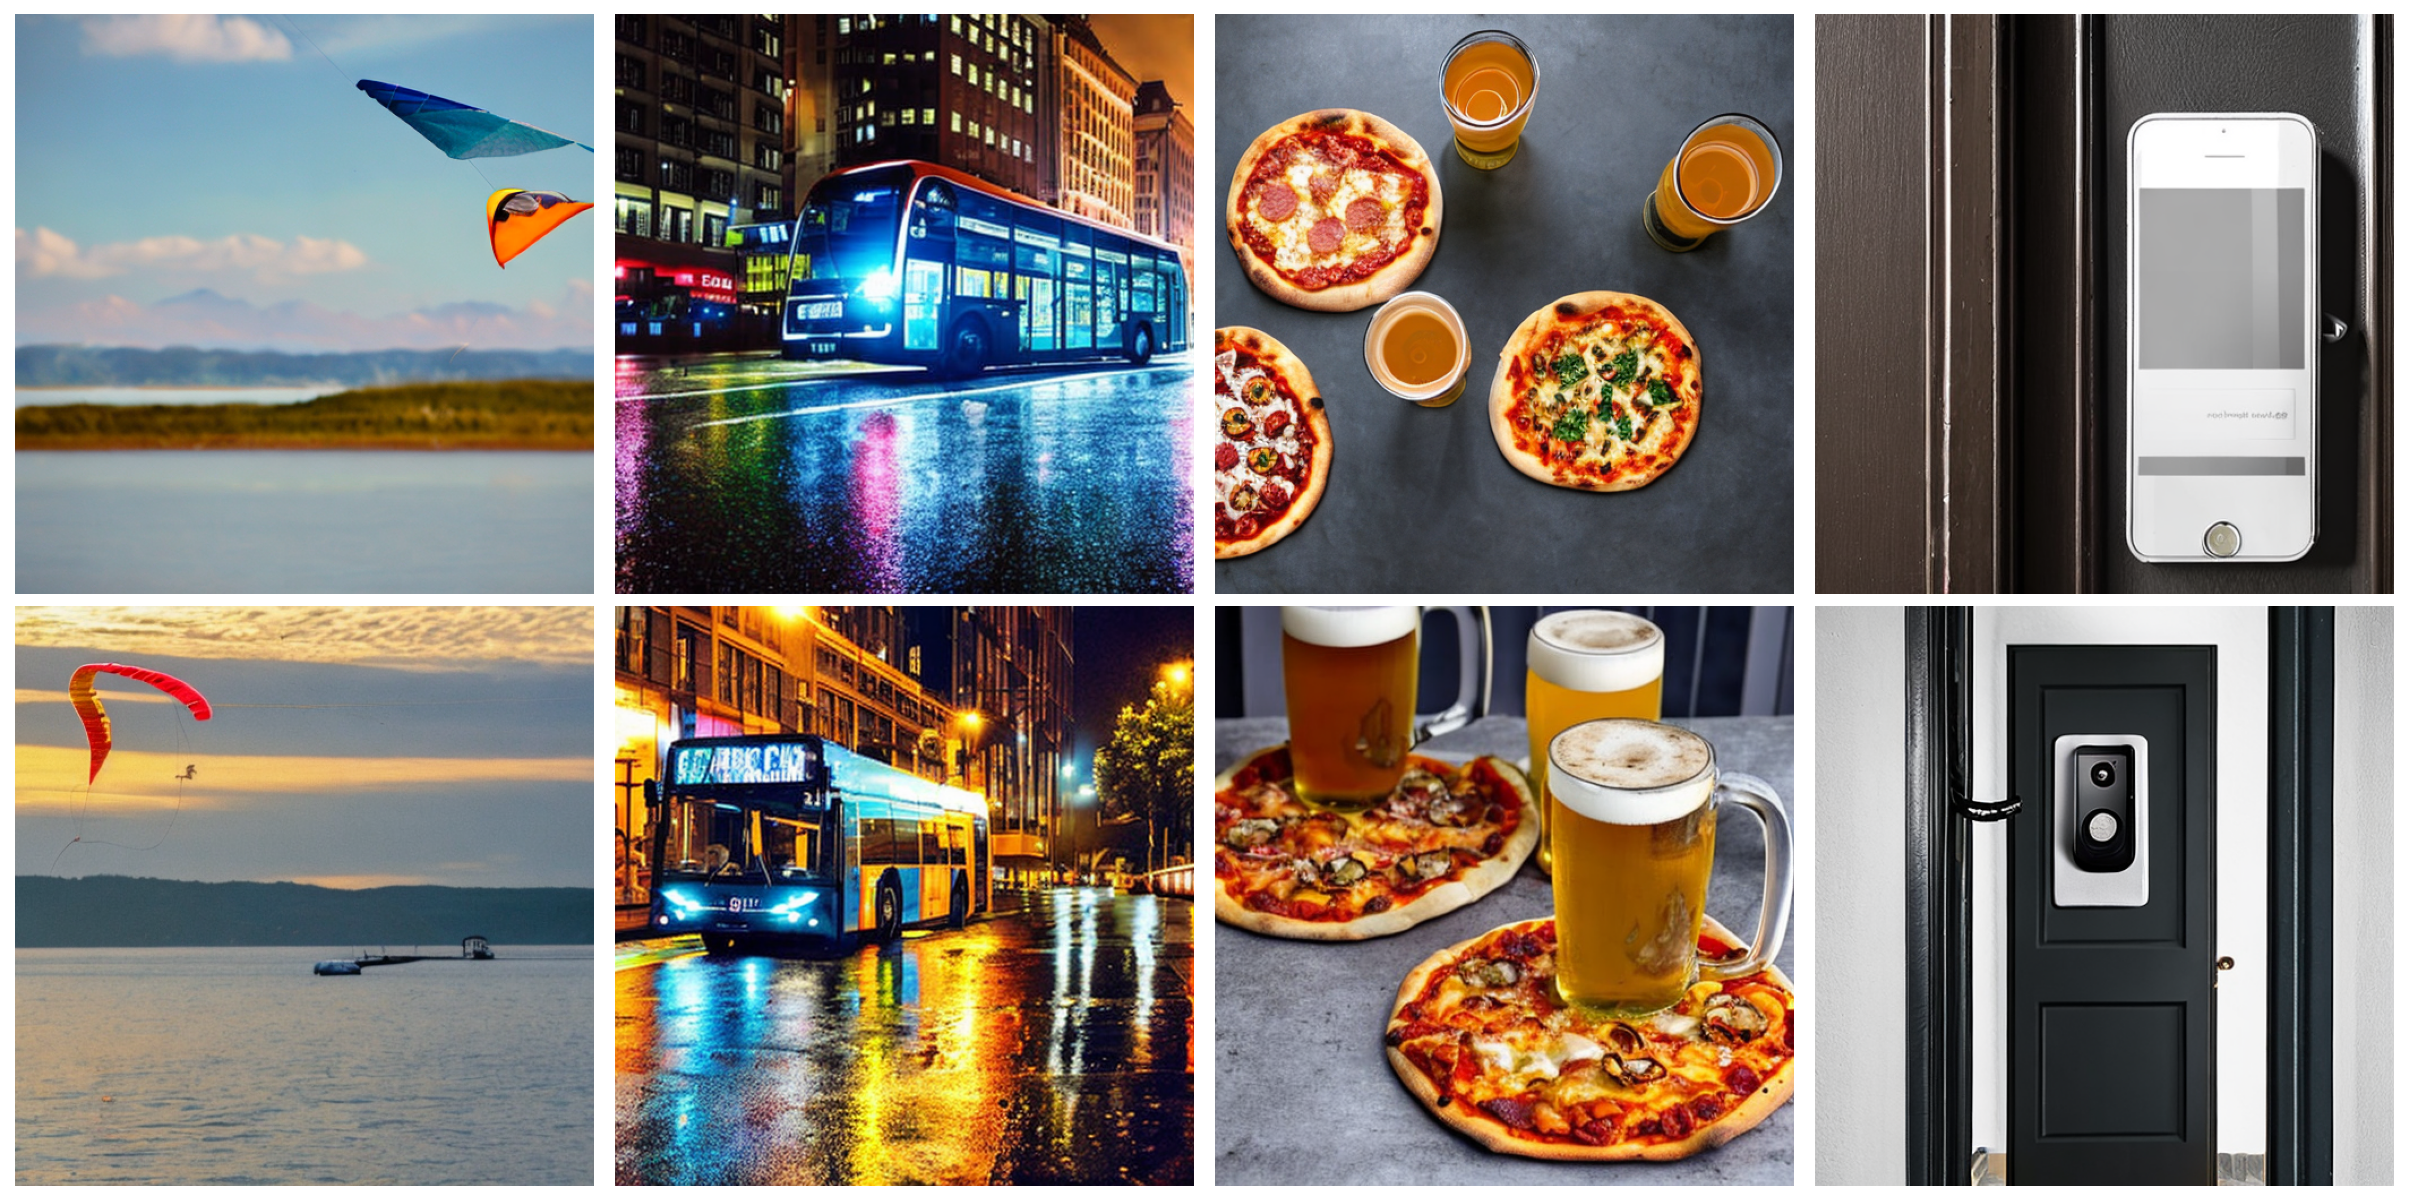
\includegraphics[width=\textwidth]{assets/visual_comparison.pdf}
    \caption{Visual comparison of non-watermarked (top row) and watermarked (bottom row) images. No perceptible visual difference is observed across a range of styles and subjects.}
    \label{fig:visual_comparison}
\end{figure}

\section{Robustness Evaluation}
The second phase of the evaluation tested the watermark's resilience against a suite of 12 common digital attacks. The primary metric was the \ac{BER}, with lower values indicating higher robustness.

The results, summarised in Table \ref{tab:robustness_summary}, demonstrate that Gaussian Shading is highly robust against most signal processing attacks. As shown in Figure \ref{fig:robustness_jpeg_noise}, the watermark maintains a \ac{BER} below 0.015 even under severe \ac{JPEG} compression (quality factor of 25) and significant Gaussian noise ($\sigma=0.05$). This performance exceeds the success criteria defined in the methodology.

However, the evaluation revealed a critical vulnerability to geometric attacks. The random crop attack, which removed 20\% of the image area before resizing, resulted in a mean \ac{BER} of 0.4852. A \ac{BER} of 0.5 is equivalent to random chance, meaning the watermark was completely destroyed. This catastrophic failure, highlighted in Figure \ref{fig:robustness_blur_crop}, indicates that the spatial redundancy of the watermark is insufficient to survive the loss of image data from cropping.

\begin{table}[htb]
    \caption{Watermark Robustness Summary (Mean BER).}
    \label{tab:robustness_summary}
    \begin{center}
    \resizebox{\textwidth}{!}{%
    \begin{tabular}{|l|l|c||l|l|c|}
    \hline
    \textbf{Attack Type} & \textbf{Parameter} & \textbf{Mean BER} & \textbf{Attack Type} & \textbf{Parameter} & \textbf{Mean BER} \\ \hline
    \multirow{4}{*}{JPEG Compression} & Quality=90 & 0.0017 & \multirow{2}{*}{Gaussian Blur} & Radius=2 & 0.0017 \\
     & Quality=75 & 0.0028 & & Radius=4 & 0.0180 \\
     & Quality=50 & 0.0050 & \multirow{2}{*}{Brightness} & Factor=0.5 & 0.0006 \\
     & Quality=25 & 0.0135 & & Factor=2.0 & 0.0023 \\ \cline{1-3}
    \multirow{3}{*}{Gaussian Noise} & $\sigma=0.01$ & 0.0015 & \multirow{2}{*}{\textbf{Random Crop}} & \multirow{2}{*}{\textbf{80\%}} & \multirow{2}{*}{\textbf{0.4852}} \\
     & $\sigma=0.03$ & 0.0037 & & & \\
     & $\sigma=0.05$ & 0.0069 & & & \\ \hline
    \end{tabular}%
    }
    \end{center}
\end{table}

\begin{figure}[htb]
    \centering
    \includegraphics[width=\textwidth]{assets/robustness_jpeg_noise.pdf}
    \caption{Robustness against JPEG compression (left) and Gaussian noise (right). The watermark shows high resilience, with BER remaining very low even under severe attack conditions.}
    \label{fig:robustness_jpeg_noise}
\end{figure}

\begin{figure}[htb]
    \centering
    \includegraphics[width=\textwidth]{assets/robustness_blur_crop.pdf}
    \caption{Robustness against Gaussian blur (left) and a comparison of severe attacks (right). The bar chart highlights the catastrophic failure of the crop attack compared to other severe distortions.}
    \label{fig:robustness_blur_crop}
\end{figure}

\section{Discussion}
The empirical results provide a nuanced answer to the research questions. While Gaussian Shading is visually imperceptible and robust to many common attacks, its claim of being "performance-lossless" is questionable under the rigorous standard of distributional analysis (\ac{FID}). Furthermore, its vulnerability to cropping is a significant practical limitation. The trade-off is clear: the method achieves its training-free nature and high capacity at the cost of statistical purity and resilience to geometric data loss. Compared to methods like Stable Signature, it avoids costly fine-tuning, but at the expense of the deeper, more robust integration that fine-tuning provides. This positions Gaussian Shading as a valuable, easy deployment, in-generation, training free, solution for scenarios where geometric attacks, such as cropping, are not the main concern.

\chapter{Conclusion}
\label{cha:conclusion}

This dissertation conducted a rigorous, independent evaluation of the Gaussian Shading watermarking technique for \ac{AI}-generated images. By implementing the algorithm within a Stable Diffusion v2.1 framework and subjecting it to a comprehensive evaluation protocol, this project provides critical insights into its performance and practical viability.

\section{Summary of Findings}
The study's findings are summarised by directly addressing the initial research questions:

\begin{itemize}
    \item \textbf{To what extent is Gaussian Shading robust?} The method is highly robust against signal processing attacks like \ac{JPEG} compression, noise, and blurring, with \ac{BER} remaining below 2\% even under severe conditions. However, it is fundamentally not robust to geometric attacks like cropping, which completely destroys the watermark (\ac{BER} $\approx$ 0.5).
    
    \item \textbf{What is the trade-off between robustness and image quality?} The watermark is visually and semantically imperceptible, as confirmed by near-identical \ac{CLIP} scores. However, a high \ac{FID} score of 47.83 reveals a significant shift in the image distribution, challenging the method's "performance-lossless" claim from a statistical perspective.
    
    \item \textbf{How does it compare to other techniques?} Gaussian Shading offers the key advantages of being training-free (unlike Stable Signature) and having a high data capacity (unlike the 1-bit Tree-Ring). However, these benefits come at the cost of vulnerability to cropping and a measurable impact on the output distribution.
\end{itemize}

\section{Limitations and Future Work}
This study was subject to several limitations. The evaluation was performed on a single generative model, and the \ac{FID} score calculation was based on a smaller dataset than the original paper (1,000 vs 5,000 images for Imperceptibility analysis), which may have influenced the result. The attack suite did not include more sophisticated adversarial attacks designed specifically to target and remove watermarks.

Future work should focus on three key areas. First, investigating techniques to improve robustness against geometric attacks, potentially by integrating error-correction codes such as \ac{BCH} codes to allow for watermark recovery even with partial data loss. Second, exploring modifications to the watermark embedding process to mitigate the large shift in the \ac{FID} score while preserving robustness, perhaps through a more advanced sampling strategy. Finally, the technique should be evaluated across a wider range of generative models and against adversarial attacks to fully assess its security in real-world scenarios.

\section{Final Remarks}
In conclusion, this project confirms that Gaussian Shading is a promising, easy-to-deploy watermarking solution with high imperceptibility and strong robustness to many common image alterations. However, this independent evaluation has also identified and quantified critical weaknesses—namely, its failure to withstand cropping and its significant impact on the statistical distribution of generated images. These findings represent a valuable contribution to the field, providing a more complete and critical understanding of the trade-offs inherent in this state-of-the-art technique and highlighting important directions for the development of future watermarking solutions for responsible \ac{AI}.

\appendix
\chapter{Additional Results and Implementation Details}
\label{app:AdditionalContent}

\section{Key Algorithm Implementation}
This section provides the Python code for the core distribution-preserving sampling function, which is the central innovation of the Gaussian Shading technique.

\begin{lstlisting}[language=Python, caption={Distribution-Preserving Sampling Implementation}]
def distribution_preserving_sampling(z_t, m, alpha=0.5):
    # Convert to uniform using normal CDF
    u_z = 0.5 * (1 + torch.erf(z_t / math.sqrt(2)))
    
    # Create reference latent based on watermark bit
    z_ref = torch.randn_like(z_t)
    u_ref = 0.5 * (1 + torch.erf(z_ref / math.sqrt(2)))
    
    # Adjust reference values based on watermark bits
    mask = (m > 0.5).float()
    u_ref = mask * torch.clamp(u_ref, min=0.5) + (1 - mask) * torch.clamp(u_ref, max=0.5)
    
    # Interpolate in uniform space
    u_mix = alpha * u_z + (1 - alpha) * u_ref
    
    # Convert back to normal distribution
    # Clamp to avoid numerical issues at extremes
    u_mix_safe = torch.clamp(u_mix, min=1e-6, max=1-1e-6)
    z_watermarked = math.sqrt(2) * torch.erfinv(2 * u_mix_safe - 1)
    
    return z_watermarked
\end{lstlisting}

\section{Full Robustness Data}
Table \ref{tab:full_robustness_data} provides the complete summary of the robustness evaluation, including the mean accuracy and mean Bit Error Rate (BER) for all 12 attack configurations performed on the 200-image test set.

\begin{table}[htb]
\caption{Complete Robustness Evaluation Summary.}
\label{tab:full_robustness_data}
\begin{center}
\begin{tabular}{|l|c|c|c|}
\hline
\textbf{Attack Name} & \textbf{Attack Parameter} & \textbf{Mean Accuracy} & \textbf{Mean BER} \\
\hline
brightness & 0.50 & 0.9994 & 0.0006 \\
brightness & 2.00 & 0.9977 & 0.0023 \\
crop & 0.80 & 0.5148 & 0.4852 \\
gaussian\_blur & 2.00 & 0.9983 & 0.0017 \\
gaussian\_blur & 4.00 & 0.9820 & 0.0180 \\
gaussian\_noise & 0.01 & 0.9985 & 0.0015 \\
gaussian\_noise & 0.03 & 0.9963 & 0.0037 \\
gaussian\_noise & 0.05 & 0.9931 & 0.0069 \\
jpeg & 25.00 & 0.9865 & 0.0135 \\
jpeg & 50.00 & 0.9950 & 0.0050 \\
jpeg & 75.00 & 0.9972 & 0.0028 \\
jpeg & 90.00 & 0.9983 & 0.0017 \\
\hline
\end{tabular}
\end{center}
\end{table}

\chapter{Ethics Checklist}
\label{app:EthicsChecklist}
\section*{Ethical Considerations Checklist and Declaration}

\subsection*{Project Description}
\textit{Briefly explain the methodology of your study. Give sufficient detail that a non-expert in the subject can understand what you are proposing to do.}

\vspace{1em}
\noindent
\begin{tabularx}{\textwidth}{|X|}
\hline
Identifying images generated by Artificial Intelligence (AI) with invisible watermarks: This can help improve copyright protections, traceability, and accountability. A watermarking method will be implemented to embed and retrieve these imperceptible watermarks with minimal compromise to quality. The method will be evaluated against its resistance to common attacks such as compression, cropping, noise, and smoothing. Additionally the chosen method will be compared with existing methods. \\
\hline
\end{tabularx}

\subsection*{External Datasets}
\textit{If you are using external datasets, please (a) identify the dataset(s) giving sufficient details; (b) identify the relevant licence or terms of use for the dataset(s) and justify why your project would be compliant with those terms; (c) if the data is about humans, also provide evidence that the data was initially collected with consent.}

\vspace{1em}
\noindent
\begin{tabularx}{\textwidth}{|X|}
\hline
The project will make use of text-to-image prompt datasets in order to have standardisation of generated images COCO-2017 (CC BY-SA 4.0), Meaning attribution is required. The project will be compliant with the terms as no changes are being made and the datasets used will be credited and referenced Gustavosta prompt set. \\
\hline
\end{tabularx}

\subsection*{Potential Ethical Issues}
\textit{Does your project involve any of the following? Please mark Yes or No for \textbf{all} issues.}

\vspace{1em}
\noindent
\begin{tabularx}{\textwidth}{|X|c|}
\hline
\textbf{Issue} & \textbf{Yes / No} \\
\hline
Human participants (adults or children) & No \\
\hline
Human data (e.g. data collected through surveys and questionnaires on issues such as lifestyle, housing and working environments, or attitudes and preferences, or datasets including human data) & No \\
\hline
Datasets that require permission from the data provider & No \\
\hline
Applications that could potentially involve unethical practice, including potential dual-use applications (e.g. projects involving tools or data that can be used for unethical purposes e.g. to attack systems) & No \\
\hline
Funding sources or collaboration with potential to adversely affect existing relationships or bring the University or Department into disrepute (e.g. projects related to gambling, dark market, etc.) & No \\
\hline
Restrictions on dissemination (e.g. not being allowed to publish certain datasets or results) & No \\
\hline
Military or defence context & No \\
\hline
Overseas countries under regimes with poor human rights record or identified as dangerous by the Foreign \& Commonwealth Office & No \\
\hline
Human material (e.g. tissue or fluid samples), vertebrates, especially mammals and birds, or any other organisms not previously mentioned & No \\
\hline
\end{tabularx}

\vspace{1em}
\noindent
\textit{If you answered \textbf{No} to all the above, you do not need ethical approval.}

\vspace{1em}
\noindent
\textit{If you answered \textbf{Yes} to any of the above, you must complete a Fast-Track Ethical Approval Form, get it signed off by your project advisor, and submit it for approval to the Departmental Ethics Officers.}

\subsection*{Student Declaration}
\textit{I have considered the ethical implications of this project, all the terms and conditions and permissions of any datasets being used, and I have identified no significant ethical implications requiring an ethical approval application.}

\vspace{1em}
\noindent
\begin{tabularx}{\textwidth}{|l|X|}
\hline
\textbf{Student Name} & Mischa Zaynchkovsky \\
\hline
\textbf{Student Signature} & Mischa Zaynchkovsky \\
\hline
\textbf{Date} & 14/02/2025 \\
\hline
\end{tabularx}

\sloppy % relax spacing between words
\printbibliography

\end{document}
